\documentclass{article}
\usepackage[utf8]{inputenc}
\usepackage[portuguese]{babel}
\usepackage[a4paper, total={7in, 9in}]{geometry}
\usepackage{graphicx}
\usepackage{float}
\usepackage{verbatim}
\usepackage[bottom]{footmisc}
\usepackage[style=numeric]{biblatex}
\usepackage{minted}
\usepackage{csquotes}
\usepackage{fancyvrb}
\usepackage[title]{appendix}
\usepackage{xcolor}
\usepackage{indentfirst}
\usepackage{svg}
\addbibresource{references.bib}

\newcommand{\titleRule}{
    \rule{\linewidth}{0.5mm} \\ [0.25cm]
}

\begin{document}

{
\center
\textsc{\Large Universidade do Minho} \\ [0.5cm]
\textsc{\Large Mestrado Integrado em Engenharia Informática} \\ [0.5cm]
\textsc{\large Engenharia de Sistemas de Computação} \\ [0.5cm]

{\LARGE \bfseries Implementação paralela do algoritmo Heap Sort} \\[0.2cm]

\begin{tabular}{c c}
    José Carlos Lima Martins & Miguel Miranda Quaresma \\
    A78821 & A77049  \\
\end{tabular} \\[0.5cm]

\today \\[1cm]
}



\section{Introdução}
A ordenação de conjuntos de valores possui aplicações nas mais diversas áreas da computação envolvendo, frequentemente, listas
de tamanho considerável. Por forma a permitir a ordenação em tempo útil destes conjuntos é imperativo recorrer a algoritmos 
eficientes do ponto de vista computacional, que diferem nas estruturas de dados usadas para ordenar listas. 
Adicionalmente, torna-se útil em certos casos, a implementação destes algoritmos em paradigmas de computação paralela, permitindo
tirar partido do poder computacional disponível nos processadores modernos. Esta implementação influencia diretamente o algoritmo
escolhido dado que nem todos são propícios a serem paralelizados dadas as estruturas e dependências de dados que apresentam.
Como tal, o presente trabalho prende-se com esta segunda fase, mais concretamente, com a implementação paralela, num paradigma de memória 
partilhada, do algoritmo \textit{Heap Sort}, que recorre a uma estrutura de dados do tipo \textit{(max) heap} para ordenar um conjunto de 
valores por ordem crescente. Para determinar se é vantajoso paralelizar este algoritmo são analisadas três versões do mesmo, uma versão 
sequencial e duas versões paralelas desenvolvidas com recurso à biblioteca \textit{Pthreads}, sendo analisada a escalabilidade das mesmas
face a um conjunto de parâmetros como o tamanho do conjunto de valores a ser ordenado e o número de \textit{threads} usadas.
Para esta análise será ainda usado o perfil de execução de cada uma das versões, permitindo assim identificar que fatores limitam (ou não)
a escalabilidade das implementações em questão.

\section{Implementações}
A análise de escalabilidade realizada compara os tempos de execução de duas implementações paralelas do algoritmo \textit{Heap Sort} com a versão
sequencial do mesmo algoritmo. Estas duas versões diferem na granularidade das zonas críticas existentes \textbf{i.e.} no número de zonas de 
exclusão, que altera o número de \textit{threads} que podem estar em execução (paralela) num determinado instante. É importante realçar que, no
presente algoritmo, a região crítica compreende a remoção do maior elemento da \textit{heap}, num dado instante, e subsequente inserção do mesmo
na lista ordenada bem como a função (\texttt{shiftDown\_Seq} e \texttt{shiftDown\_Par}) que permite garantir que a lista desordenada mantém a propriedade 
de \textit{max heap}.
Para permitir uma interpretação dos resultados apresentados serão descritas, de seguida, cada uma das abordagens referidas.

\subsection{Exclusão da árvore}
A primeira das versões paralelas desenvolvida realiza exclusão ao nível da \textit{heap} inteira, impedindo que mais que uma \textit{thread} leia ou 
escreva a mesma num dado instante. Para conseguir garantir exclusão mútua ao nível da árvore é usado um \textit{mutex} para 
mediar a entrada na região crítica:

\footnotesize
\begin{verbatim}
pthread_mutex_lock(&tree_lock); 
if(end > 0){
    int cmax = a[0];
    a[0]=a[end];
    a[end]=cmax;
    end--;
    shiftDown_Seq(a,0,end);
    pthread_mutex_unlock(&tree_lock);
}else{
    pthread_mutex_unlock(&tree_lock);
    break;
}
\end{verbatim}
\normalsize
que também media o acesso à variável partilhada \texttt{end}. A função \texttt{shiftDown\_Seq} realiza a correção da \textit{heap} após 
ter sido removido o maior valor da mesma, de maneira a que esta mantenha a propriedade de \textit{max heap}. Uma característica importante 
desta abordagem prende-se com o facto da mesma ser equivalente à versão sequencial no sentido em que a função \texttt{shiftDown\_Seq} é sempre 
realizada sequencialmente. Como tal, esta abordagem apresenta poucas vantagens quanto ao paralelismo explorado, envolvendo a complexidade 
adicional de gerir primitivas como \textit{mutexes} para controlar as regiões críticas.

\subsection{Exclusão em cada nível da árvore}
A segunda versão paralela desenvolvida permite uma granularidade mais fina, implementando exclusão em cada nível da \textit{heap}. 
Para tal, é declarado um \textit{array} de \textit{mutexes} que controlam o acesso a cada um destes níveis. Sendo assim, o \textit{array}
contém tantos elementos quanto a altura da \textit{heap}: 

\footnotesize 
\begin{verbatim}
level_count = ceil(log(size) / log(2));
...
level_locks = (pthread_mutex_t*)malloc(level_count * sizeof(pthread_mutex_t));
\end{verbatim}
\normalsize
Esta abordagem permite que exista mais que uma \textit{thread} a realizar operações sobre a \textit{heap}, desde que em níveis distintos.
Quando uma dada \textit{thread} pretende remover o maior elemento da \textit{heap}, esta realiza o \textit{lock} do \textit{mutex} correspondente
ao nível 0, requisitando ainda o \textit{lock} para escrita da variável \texttt{end}, que é mediada por um \textit{Read-Write Lock}. 
O uso de uma primitiva deste tipo para a variável \textit{end} permite que várias \textit{threads} realizem o \texttt{shiftDown} de um valor 
(que designaremos \textbf{alvo}) garantindo, ao mesmo tempo, que apenas uma pode retirar o valor máximo da \textit{heap} num dado instante e 
que este valor não é sobre-escrito por uma \textit{thread} a realizar o \texttt{shiftDown}. Após a \textit{thread} inserir o novo valor na 
lista ordenada, trocando-o com o alvo da função \textit{shiftDown}, esta liberta o \textit{lock} para escrita da variável \texttt{end} mas 
mantém o \textit{lock} do nível 0 da \textit{heap}, por forma a impedir que outra \textit{thread} retirasse o alvo da primeira posição (nível) 
da \textit{heap} e o inserisse na lista ordenada, sem que este correspondesse ao maior valor da \textit{heap}. Como tal, o \textit{lock} do 
nível 0 apenas é liberto quando a \textit{thread} que inseriu o último valor na lista ordenada realiza a primeira operação de \texttt{shiftDown} 
sobre o alvo, instante após o qual a primeira posição contém o maior valor da "nova" \textit{heap}. A operação de \texttt{shiftDown} exige que 
cada \textit{thread} tenha acesso exclusivo aos dois níveis que manipula, aquele onde se encontra o alvo e o nível seguinte, para onde este 
será movido de seguida. Como tal, cada \textit{thread} mantém sempre o \textit{lock} do nível onde se encontra alvo e realiza o \textit{lock} 
do nível seguinte a cada iteração do ciclo. Adicionalmente, como nenhuma das \textit{threads} altera a variável \texttt{end} na função 
\texttt{shiftDown}, estas apenas realizam o \textit{lock} para leitura da mesma. Este \textit{lock} apenas é requisitado quando a \textit{thread} já 
possui acesso aos dois níveis que necessita, garantindo que não ocorre um \textit{dead lock}. Isto permite também garantir que a ordem de 
invocação da função \texttt{shiftDown\_Par} é mantida, dado que uma \textit{thread} apenas pode avançar para o nível seguinte quando o 
\textit{lock} do mesmo for libertado. A abordagem descrita permite que a função \texttt{shiftDown\_Par} seja executada, em paralelo, por 
$\frac{h}{2}$ \textit{threads}, onde $h$ corresponde à altura da \textit{heap}.

\section{Resultados}

\subsection{Contexto de experimentação} \label{context}
Os testes foram realizados na máquina com configurações apresentadas em \ref{hardware}, e usaram como parâmetros para o tamanho da \textit{heap}:
\begin{itemize}
    \item 8192 (que cabe na \textit{cache} L1) 
    \item 65536  (que cabe na \textit{cache} L2) 
    \item 1572864 (que cabe na \textit{cache} L3) 
    \item 3145728 (que apenas cabe em memória) 
\end{itemize}
As versões \textit{multithreaded} foram testadas com 2, 4, 8 e 16 \textit{threads}.

O código (fonte) foi compilado com a versão 8.3.0 do compilador GCC com a \textit{flag} de otimização \texttt{-O2}.

Por forma a obter valores normalizados, precisos, reproduzíveis e limitar a influência de \textit{outliers} nos valores considerados foram
recolhidas, para cada teste, 15 amostras e o valor da mediana tomado como o tempo de execução para a configuração 
correspondente.

Por fim, foi também usada a ferramenta \texttt{perf} por forma a, em primeiro lugar obter algumas estatísticas de contadores, através do \texttt{perf stat} e, em segundo lugar, para obter a \texttt{call stack} de cada versão, com recurso a \texttt{perf record} e \texttt{perf report}.

\subsection{Análise dos resultados}

Os resultados de \textit{speed up} obtidos em cada uma das abordagens, presentes no gráfico \ref{fig:speed_up}, permitem verificar uma perda de 
\textit{performance} nas versões paralelas relativamente à versão sequencial. Esta observação advém da necessidade das versões paralelas mediarem o 
acesso das \textit{threads} a zonas críticas, levando a que estas passem grande parte do seu tempo à espera para obter acesso a estas zonas. Adicionalmente, a gestão destas zonas através de primitivas como \textit{mutexes} e \textit{read-write locks} introduz
um \textit{overhead} que limita ainda mais os ganhos obtidos. Esta perda de \textit{performance} deve-se ao número considerável de dependências 
de dados existentes no algoritmo \textit{Heap Sort}, que requer um controlo de concorrência rigoroso e impede ganhos na \textit{performance}. 

Ainda através do mesmo gráfico, percebe-se que a versão paralela com exclusão da árvore tem melhor performance que a versão 
paralela com exclusão por níveis da árvore, devido ao facto já referido, a segunda possui mais zonas de exclusão (apesar de 
mais pequenas) que precisam de ser mediadas, obrigando a um maior número de \textit{locks} e \textit{unlocks} bem como a um 
maior número de mecanismos de controlo (\textit{mutexes} e \textit{read-write locks}).

Para além disso, na versão paralela com exclusão por níveis observa-se que, quanto maior o tamanho do \textit{array}, melhor 
é a \textit{performance} obtida, devido ao facto de que este aumento no número de elementos resulta num aumento da altura da 
árvore que permite que mais \textit{threads} estejam em execução paralela nos diferentes níveis da árvore.

Por outro lado, através das instruções por ciclo, gráfico disponível em \ref{fig:inst_per_cycle}, é possível identificar o 
aproveitamento que cada abordagem faz dos recursos disponíveis, neste caso o CPU. Nomeadamente, quanto maior for o número de 
instruções por ciclo, maior será o uso de CPU. Com esta métrica seria também possível saber a percentagem de utilização do CPU, 
que pode ser calculada pela razão entre o número de instruções por ciclo e o número de instruções que o CPU é capaz de lançar por 
ciclo \cite{cpuUtili}. Tendo estes fatores em conta, é possível identificar que a versão sequencial apresenta uma utilização de CPU 
maior em relação às versões paralelas. Por outro lado, das versões paralelas desenvolvidas, a que apresenta granularidade ao nível 
da árvore apresenta, com 2 \textit{threads}, uma maior utilização do CPU que a versão paralela com exclusão por níveis da árvore. 
Contudo, para valores superiores a 2 \textit{threads}, esta relação tem tendência a inverter-se, registando-se uma maior utilização 
do CPU por parte da versão que implementa exclusão em cada nível da árvore, algo que corrobora o que foi referido anteriormente.

\subsection{Perfil de Execução}
O perfil de execução de um dado processo permite identificar a percentagem de tempo que cada secção do mesmo ocupa, face ao tempo
total de execução. Como tal, este representa uma informação imprescindível quando se pretende perceber que secções podem ser otimizadas
ou quais as que são responsáveis pela maior "fatia" de tempo total. 
A obtenção deste perfil foi conseguida utilizando a ferramenta \texttt{perf}, nomeadamente às funcionalidades \texttt{record}, para recolher os dados referentes à execução do programa, e \texttt{report} que processa estes dados de forma a que sejam passíveis
de ser interpretados.

Os dados relativos ao perfil de execução da versão paralela com exclusão ao nível da árvore recolhidos pela ferramenta \texttt{perf} 
(ver \ref{execprofile_tree_raw}) foram agregados no gráfico \ref{fig:execprofile_tree} para ser possível perceber de que forma
os parâmetros de execução (tamanho da lista e número de \textit{threads}) influenciam o perfil de execução desta versão. 

Atentando às alterações que um aumento no tamanho da lista introduz no comportamento desta versão é possível verificar que, como esperado,
a percentagem de tempo correspondente à função \texttt{shiftDown\_Seq} aumenta entre 5\% a 6\%, mesmo tendo em conta que o tempo total de
execução aumenta. Isto deve-se ao facto da altura da \textit{heap} aumentar e, como tal, exigir que sejam realizadas mais iterações na 
função \texttt{shiftDown\_Seq} para que um valor seja corretamente (re)colocado na \textit{heap}.

Por outro lado, para um dado tamanho da lista, é possível verificar outro comportamento interessante, o aumento no número de \textit{threads}
resulta, em ambos os casos presentes no gráfico \ref{fig:execprofile_tree}, num aumento na percentagem de tempo referente a \textit{lock's} e 
\textit{unlock's}, aumento este que ronda os 10\%. Mais uma vez, este comportamento é facilmente justificado pelo facto de, como existem mais
\textit{threads} a tentar entrar na região crítica, e como cada \textit{thread} tem a sua \textit{stack}, o número de vezes que a chamada a 
funções referentes a \textit{mutexes} se encontra na \textit{stack} será superior já que, como apenas uma \textit{thread} pode estar na região crítica
num dado instante, existirão mais \textit{threads} à espera de entrar nesta mesma região.

O perfil de execução da versão paralela com exclusão em cada nível da árvore, presente no gráfico \ref{fig:execprofile_level}, permite retirar 
algumas conclusões interessantes. Apesar das mudanças verificadas no perfil de execução não apresentarem diferenças tão significativas como 
na versão anterior, é importante realçar, por exemplo, a influência que o aumento no número de \textit{threads} tem na percentagem de tempo
referentes a \textit{locks/unlocks} dos \textit{mutexes} que controlam o acesso aos níveis. Este facto é esperado dado que existem mais \textit{threads}
a tentar aceder às diferentes regiões críticas correspondentes aos níveis da \textit{heap}, levando a que o número das mesmas que se encontra em 
espera aumente.  Adicionalmente, este aumento no número de \textit{threads} implica também uma diminuição na percentagem de tempo referente 
a \textit{locks/unlocks} do \textit{Read-Write Lock}, justificado pela ordem em que são realizadas as operações de \textit{lock}, sendo esta realizada
após uma \textit{thread} ter acesso ao nível que pretende manipular. Como este acesso é mais difícil, derivado do aumento no número de \textit{threads}, 
verifica-se uma diminuição na percentagem de tempo passado à espera de obter acesso ao \textit{Read-Write Lock}. É ainda importante realçar que 
este aumento no número de \textit{threads} implica uma diminuição da percentagem de tempo correspondente à função \texttt{shiftDown\_Par}, algo que é
esperado visto que o controlo de concorrência inerente a estas operações ocupa uma maior "fatia" de tempo.
Uma conclusão importante, referente à influência do tamanho da lista inicial, prende-se com o facto de este não alterar o perfil de execução desta versão
de maneira significativa, que justifica os ganhos no \textit{speed up}.

\subsection{Comparação das diferentes versões}

Previamente a serem realizadas comparações entre as versões é importante analisar o perfil de execução da versão sequencial para os mesmos parâmetros de 
tamanho dos perfis anteriores. Um dos aspetos a salientar no perfil de execução desta versão (ver \ref{fig:execprofile_seq}) prende-se com o aumento da 
percentagem de tempo de cerca de 5\% da função \texttt{shiftDown\_Seq} do segundo maior para o caso com o maior tamanho. Este comportamento deve-se 
claramente ao número de elementos a ordenar ser maior, o que influencia a função \texttt{shiftDown\_Seq} visto que é responsável por manter a propriedade 
de \texttt{max heap}, percorrendo grande parte, por vezes toda a \texttt{heap}.

Comparando a versão sequencial e as duas versões paralelas é possível identificar que o maior limitador de \textit{performance} das versões paralelas é a 
dependência entre os elementos da \textit{heap}, que impede que várias \textit{threads} trabalhem em paralelo na \textit{heap} de maneira a que, o \textit{overhead} 
introduzido pelo controlo de concorrência seja compensado pelo paralelismo.
Por fim, o perfil de execução da versão com exclusão em cada nível corrobora as conclusão do \textit{speed up} observado, visto que não se 
registam alterações significativas no mesmo quando se variam os parâmetros de execução e, como tal, o \textit{speed up} para um maior número de 
\textit{threads} ``aumenta''.

\section{Conclusão}
O desenvolvimento de aplicações paralelas em ambientes de memória partilhada requer a implementação de mecanismos de controlo que permitam 
garantir que as dependências de dados existentes não resultam em \textit{race conditions} que ponham em causa a correção de um dado algoritmo.
Como consequência destes mecanismos, determinados algoritmos apresentam baixo potencial para paralelização, dado que os custos de 
impedir \textit{race conditions} superam os benefícios introduzidos pelo paralelismo que, muitas vezes, é limitado ou inexistente dados os 
controlos de concorrência existentes.
As versões analisadas apresentam diferentes níveis de granularidade no que respeita ao número de regiões críticas, que influencia diretamente a
complexidade e escalabilidade de um algoritmo para problemas de tamanho superior. No entanto, é importante realçar que existe outra abordagem 
que permite obter um nível de granularidade superior mas que exige um maior controlo de concorrência. Esta abordagem consiste em associar a
cada elemento da \texttt{heap} o seu próprio \texttt{mutex}. A partir destes \texttt{mutexes}, e de forma a garantir a manutenção de um estado 
consistente da \textit{heap}, sempre que uma \texttt{thread} pretendesse realizar a operação \textit{shift down} de um elemento, necessitaria 
de obter o \texttt{lock} de ambos os filhos desse mesmo elemento (\textit{Left} e \textit{Right}). Esta abordagem permitiria que mais que uma 
\textit{thread} realizasse a operação de \textit{shift down} num dado nível da \textit{heap} desde que em "ramos" diferentes, aumentando o 
potencial de paralelismo existente. 

\printbibliography

\newpage 
\begin{appendices}

\section{Especificações do Hardware}
\label{hardware}
\begin{itemize}
    \item Fabricante: Asus
    \item Modelo: VivoBook S14 S410UN
    \item CPU:
        \begin{itemize}
            \item Fabricante: Intel
            \item Modelo: i5-8250U 1.60GHz
            \item Número de cores: 4 cores, 8 threads (Hyper-Threading)
        \end{itemize}
    \item Memória Principal:
        \begin{itemize}
            \item Tamanho: 8 GB
        \end{itemize}
    \item Hierarquia de Memória:
        \begin{itemize}
            \item Tamanho e associatividade das caches:
                \begin{itemize}
                    \item L1d (por core): 32 KiB, 8-way
                    \item L1i (por core): 32 KiB, 8-way
                    \item L2 (por core): 256 KiB, 4-way
                    \item L3 (por package): 6144 KiB, 12-way
                \end{itemize}
        \end{itemize}
\end{itemize}

\section{Resultados}

\subsection{Tempos de execução}
\begin{figure}[H]
    \centering
    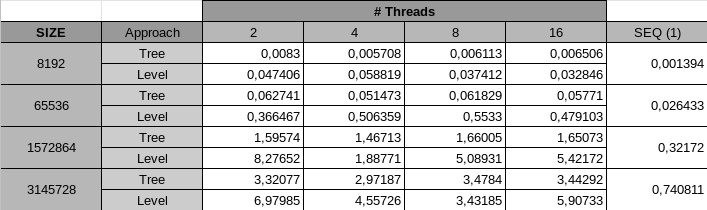
\includegraphics[width=18cm]{Pictures/tableTimes.png}
    \caption{Medianas dos tempos de execução (segundos)}
    \label{fig:table_times}
\end{figure}

\subsection{Speed-Up}
\begin{figure}[H]
    \centering
    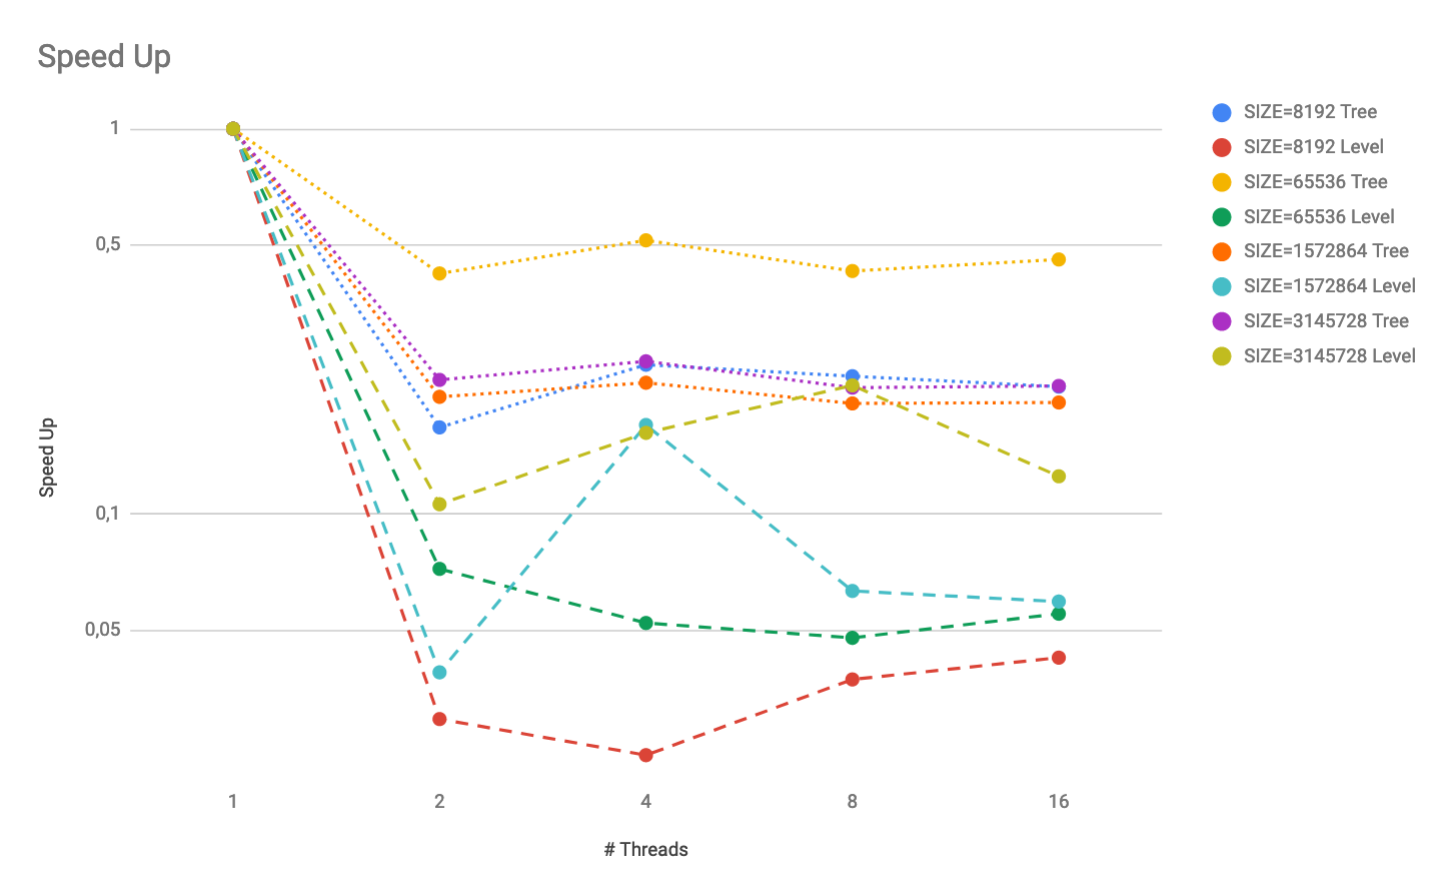
\includegraphics[width=18cm]{Pictures/SpeedUp.png}
    \caption{Speed-Up das versões paralelas}
    \label{fig:speed_up}
\end{figure}

\subsection{Instruções por ciclo}
\begin{figure}[H]
    \centering
    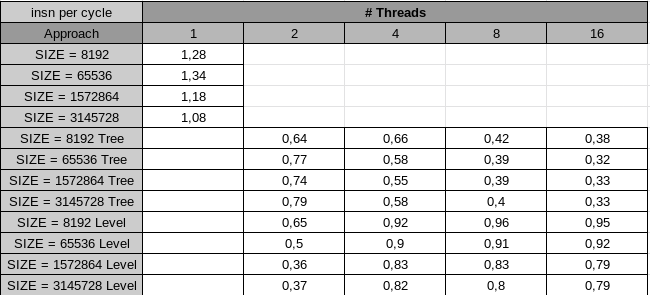
\includegraphics[width=18cm]{Pictures/tableInsPerCycle.png}
    \caption{Número de instruções por ciclo}
    \label{fig:inst_per_cycle_table}
\end{figure}

\begin{figure}[H]
    \centering
    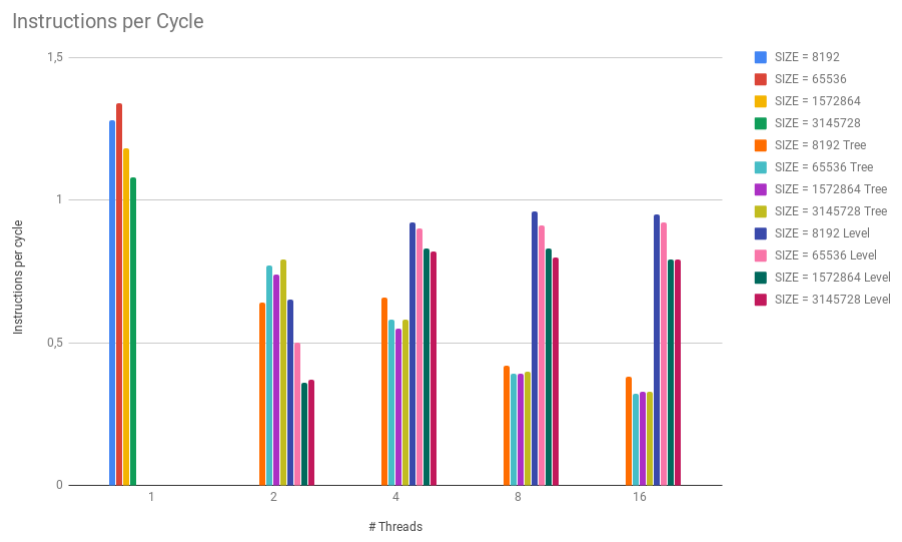
\includegraphics[width=18cm]{Pictures/InstPerCycle.png}
    \caption{Número de instruções por ciclo}
    \label{fig:inst_per_cycle}
\end{figure}
\end{appendices}

\subsection{Perfil de Execução - Valores Agregados}

\subsubsection{Versão paralela com exclusão ao nível da árvore}
\begin{figure}[H]
    \centering
    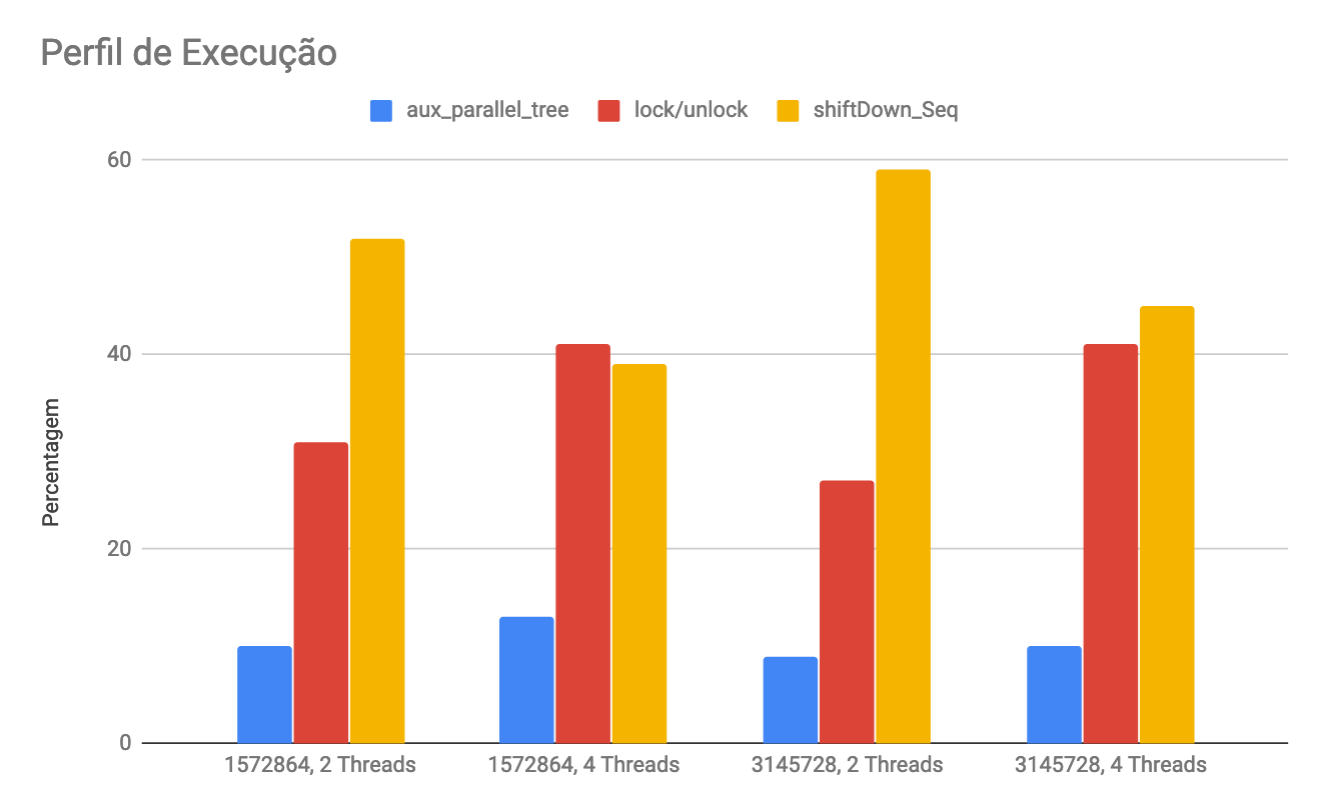
\includegraphics[width=15cm]{Pictures/ExecProfile_Tree.png}
    \label{fig:execprofile_tree}
\end{figure}

\subsubsection{Versão paralela com exclusão em cada nível da árvore}
\begin{figure}[H]
    \centering
    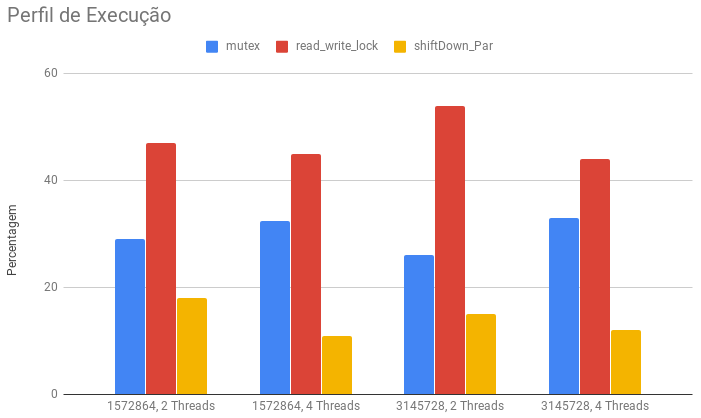
\includegraphics[width=15cm]{Pictures/ExecProfile_Level.png}
    \label{fig:execprofile_level}
\end{figure}

\subsubsection{Versão Sequencial}
\begin{figure}[H]
    \centering
    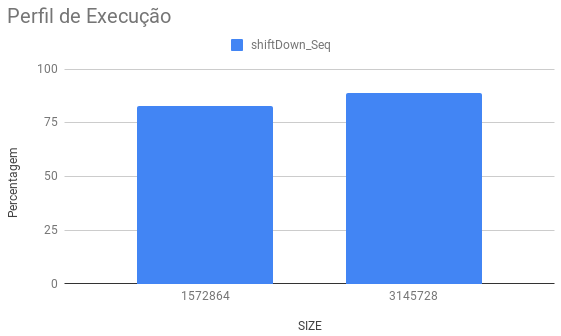
\includegraphics[width=15cm]{Pictures/ExecProfile_Seq.png}
    \label{fig:execprofile_seq}
\end{figure}

\subsection{Perfil de Execução - \texttt{Flame Graphs}}

\begin{figure}[H]
    \centering
    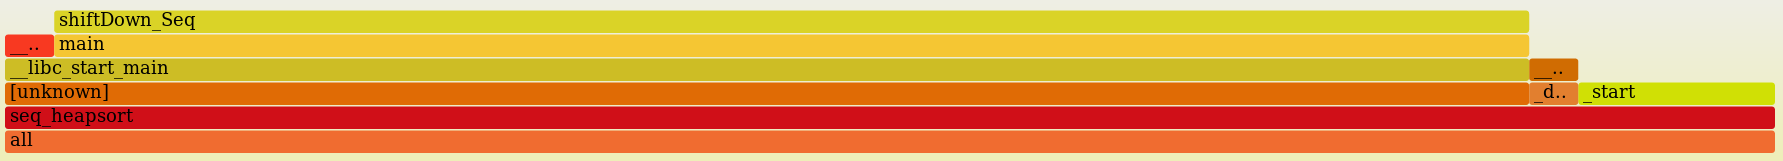
\includegraphics[width=18cm]{Pictures/seq_1572864.png}
    \caption{Versão Sequencial, 1572864 elementos}
\end{figure}

\begin{figure}[H]
    \centering
    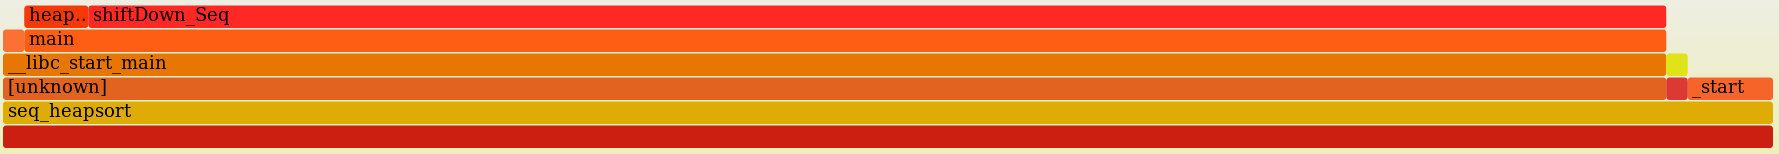
\includegraphics[width=18cm]{Pictures/seq_3145728.png}
    \caption{Versão Sequencial, 3145728 elementos}
\end{figure}

\begin{figure}[H]
    \centering
    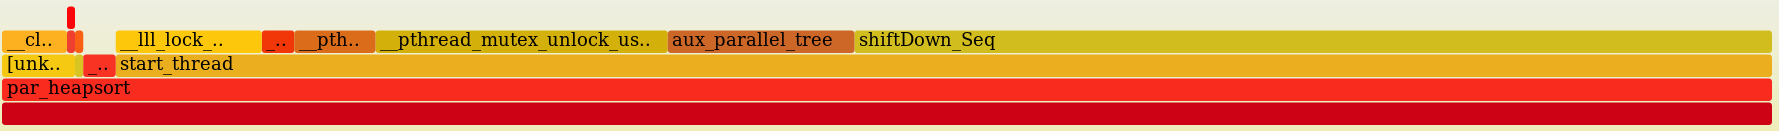
\includegraphics[width=18cm]{Pictures/par_1572864_2_tree.png}
    \caption{Versão paralela com exclusão ao nível da árvore, 1572864 elementos, 2 threads}
\end{figure}

\begin{figure}[H]
    \centering
    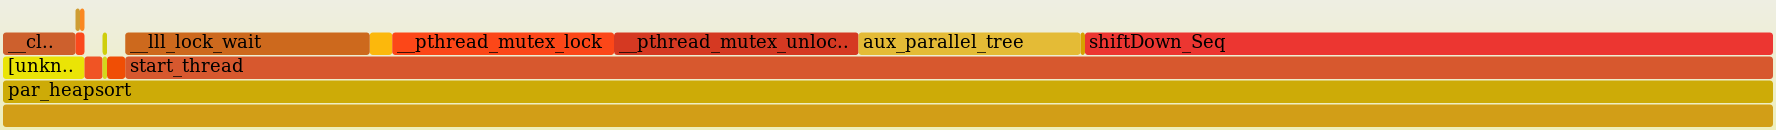
\includegraphics[width=18cm]{Pictures/par_1572864_4_tree.png}
    \caption{Versão paralela com exclusão ao nível da árvore, 1572864 elementos, 4 threads}
\end{figure}

\begin{figure}[H]
    \centering
    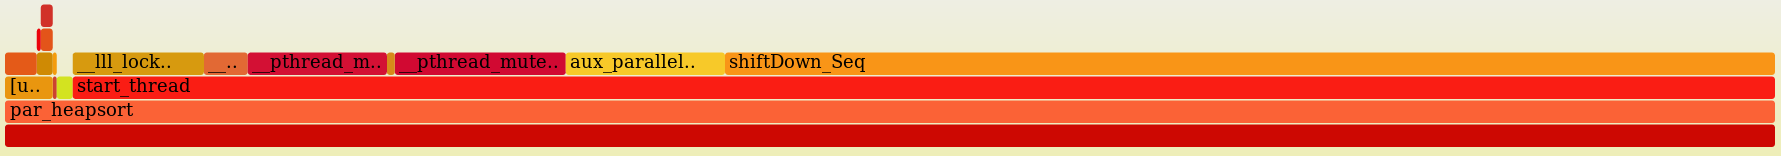
\includegraphics[width=18cm]{Pictures/par_3145728_2_tree.png}
    \caption{Versão paralela com exclusão ao nível da árvore, 3145728 elementos, 2 threads}
\end{figure}

\begin{figure}[H]
    \centering
    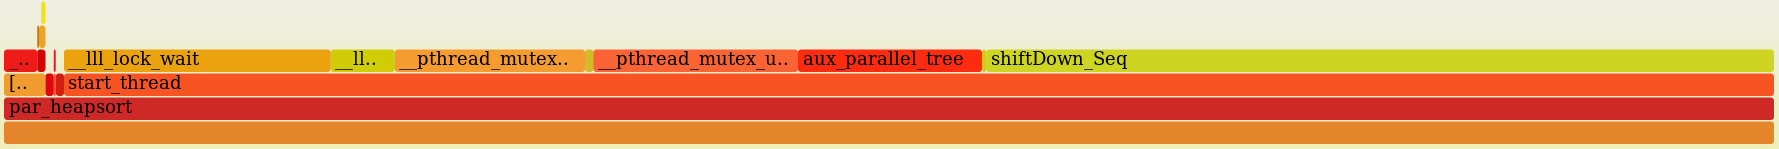
\includegraphics[width=18cm]{Pictures/par_3145728_4_tree.png}
    \caption{Versão paralela com exclusão ao nível da árvore, 3145728 elementos, 4 threads}
\end{figure}

\begin{figure}[H]
    \centering
    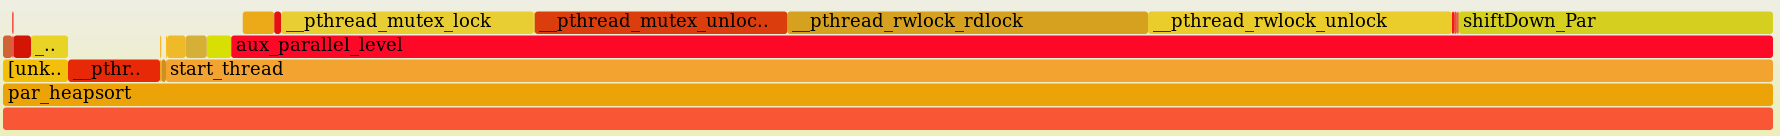
\includegraphics[width=18cm]{Pictures/par_1572864_2_level.png}
    \caption{Versão paralela com exclusão em cada nível da árvore, 1572864 elementos, 2 threads}
\end{figure}

\begin{figure}[H]
    \centering
    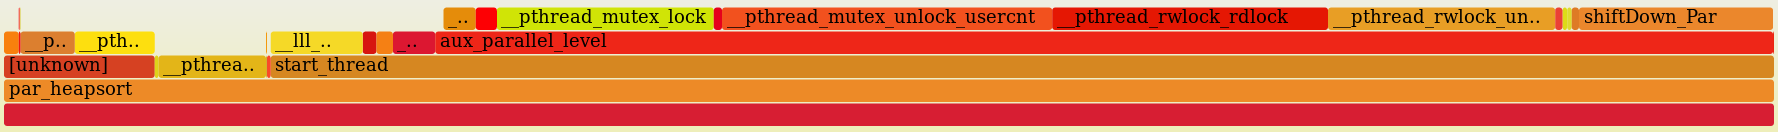
\includegraphics[width=18cm]{Pictures/par_1572864_4_level.png}
    \caption{Versão paralela com exclusão em cada nível da árvore, 1572864 elementos, 4 threads}
\end{figure}

\begin{figure}[H]
    \centering
    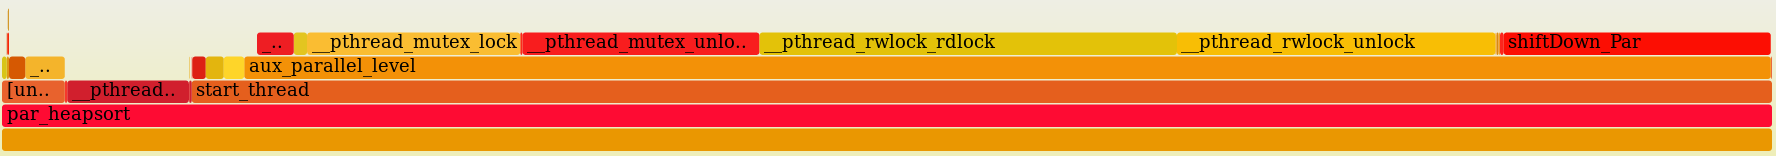
\includegraphics[width=18cm]{Pictures/par_3145728_2_level.png}
    \caption{Versão paralela com exclusão em cada nível da árvore, 3145728 elementos, 2 threads}
\end{figure}

\begin{figure}[H]
    \centering
    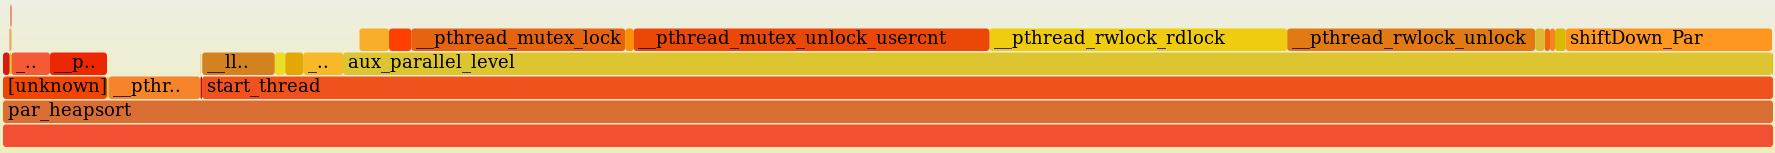
\includegraphics[width=18cm]{Pictures/par_3145728_4_level.png}
    \caption{Versão paralela com exclusão em cada nível da árvore, 3145728 elementos, 4 threads}
\end{figure}

\subsection{Perfil de Execução - \textit{Reports}}

\subsubsection{Versão sequencial, 1572864 elementos}
\scriptsize
\begin{verbatim}
# Total Lost Samples: 0
#
# Samples: 36  of event 'cycles:u'
# Event count (approx.): 799557237
#
# Children      Self       Samples  Command       Shared Object     Symbol
# ........  ........  ............  ............  ................  ..........................
#
    98.15%     0.00%             0  seq_heapsort  [unknown]         [.] 0x5541f689495641d7
            |
            ---0x5541f689495641d7
               __libc_start_main
               |
               |--86.96%--main
               |          shiftDown_Seq
               |
                --11.19%--__random_r

    98.15%     0.00%             0  seq_heapsort  libc-2.29.so      [.] __libc_start_main
            |
            ---__libc_start_main
               |
               |--86.96%--main
               |          shiftDown_Seq
               |
                --11.19%--__random_r

    86.96%    86.96%            30  seq_heapsort  seq_heapsort      [.] shiftDown_Seq
            |
            ---0x5541f689495641d7
               __libc_start_main
               main
               shiftDown_Seq

    86.96%     0.00%             0  seq_heapsort  seq_heapsort      [.] main
            |
            ---main
               shiftDown_Seq

    11.19%    11.19%             1  seq_heapsort  libc-2.29.so      [.] __random_r
            |
            ---0x5541f689495641d7
               __libc_start_main
               __random_r

     1.84%     1.84%             1  seq_heapsort  ld-2.29.so        [.] __GI___open64_nocancel
            |
            ---_dl_map_object
               __GI___open64_nocancel

     1.84%     0.00%             0  seq_heapsort  ld-2.29.so        [.] _dl_map_object
            |
            ---_dl_map_object
               __GI___open64_nocancel

     0.01%     0.01%             4  seq_heapsort  [unknown]         [k] 0xffffffffaf400a87
     0.01%     0.00%             0  seq_heapsort  ld-2.29.so        [.] _start
\end{verbatim}
\normalsize

\subsubsection{Versão sequencial, 3145728 elementos}
\scriptsize
\begin{verbatim}
# Total Lost Samples: 0
#
# Samples: 83  of event 'cycles:u'
# Event count (approx.): 1828466930
#
# Children      Self       Samples  Command       Shared Object     Symbol
# ........  ........  ............  ............  ................  .........................
#
    99.19%     0.00%             0  seq_heapsort  [unknown]         [.] 0x5541f689495641d7
            |
            ---0x5541f689495641d7
               __libc_start_main
               |
               |--94.42%--main
               |          |
               |          |--90.84%--shiftDown_Seq
               |          |
               |           --3.58%--heap_sort
               |
                --4.77%--__random

    99.19%     0.00%             0  seq_heapsort  libc-2.29.so      [.] __libc_start_main
            |
            ---__libc_start_main
               |
               |--94.42%--main
               |          |
               |          |--90.84%--shiftDown_Seq
               |          |
               |           --3.58%--heap_sort
               |
                --4.77%--__random

    94.42%     0.00%             0  seq_heapsort  seq_heapsort      [.] main
            |
            ---main
               |
               |--90.84%--shiftDown_Seq
               |
                --3.58%--heap_sort

    92.11%    90.94%            74  seq_heapsort  seq_heapsort      [.] shiftDown_Seq
            |
            |--90.94%--0x5541f689495641d7
            |          __libc_start_main
            |          main
            |          |
            |          |--89.68%--shiftDown_Seq
            |          |
            |           --1.26%--heap_sort
            |
             --1.16%--shiftDown_Seq

     4.77%     4.77%             1  seq_heapsort  libc-2.29.so      [.] __random
            |
            ---0x5541f689495641d7
               __libc_start_main
               __random

     3.58%     2.31%             2  seq_heapsort  seq_heapsort      [.] heap_sort
            |
            |--2.31%--0x5541f689495641d7
            |          __libc_start_main
            |          main
            |          heap_sort
            |
             --1.26%--heap_sort

     1.17%     1.17%             5  seq_heapsort  [unknown]         [k] 0xffffffffaf400a87
            |
             --1.16%--0x5541f689495641d7
                       __libc_start_main
                       main
                       shiftDown_Seq

     0.80%     0.80%             1  seq_heapsort  ld-2.29.so        [.] _dl_load_cache_lookup
            |
            ---_dl_map_object
               _dl_load_cache_lookup

     0.80%     0.00%             0  seq_heapsort  ld-2.29.so        [.] _dl_map_object
            |
            ---_dl_map_object
               _dl_load_cache_lookup

     0.00%     0.00%             0  seq_heapsort  ld-2.29.so        [.] _start
\end{verbatim}
\normalsize

\subsubsection{Versão paralela com exclusão ao nível da árvore, 1572864 elementos, 2 threads}\label{execprofile_tree_raw}
\scriptsize
\begin{verbatim}
# Total Lost Samples: 0
#
# Samples: 218  of event 'cycles:u'
# Event count (approx.): 1650335186
#
# Children      Self       Samples  Command       Shared Object       Symbol
# ........  ........  ............  ............  ..................  ..................................
#
    93.04%     0.00%             0  par_heapsort  libpthread-2.29.so  [.] start_thread
            |
            ---start_thread
               |
               |--55.51%--shiftDown_Seq
               |
               |--15.71%--__pthread_mutex_unlock_usercnt
               |
               |--9.74%--aux_parallel_tree
               |
               |--5.67%--__lll_lock_wait
               |
               |--4.77%--__pthread_mutex_lock
               |
                --1.64%--__lll_unlock_wake

    55.51%    55.51%           113  par_heapsort  par_heapsort        [.] shiftDown_Seq
            |
            ---start_thread
               shiftDown_Seq

    16.10%    16.10%            37  par_heapsort  libpthread-2.29.so  [.] __pthread_mutex_unlock_usercnt
            |
            ---start_thread
               |
                --15.71%--__pthread_mutex_unlock_usercnt

     9.74%     9.35%            22  par_heapsort  par_heapsort        [.] aux_parallel_tree
            |
             --9.35%--start_thread
                       aux_parallel_tree

     5.96%     5.96%             1  par_heapsort  libc-2.29.so        [.] __random_r
            |
            ---0x5541f689495641d7
               __libc_start_main
               __random_r

     5.96%     0.00%             0  par_heapsort  [unknown]           [.] 0x5541f689495641d7
            |
            ---0x5541f689495641d7
               __libc_start_main
               __random_r

     5.96%     0.00%             0  par_heapsort  libc-2.29.so        [.] __libc_start_main
            |
            ---__libc_start_main
               __random_r

     5.67%     4.87%            13  par_heapsort  libpthread-2.29.so  [.] __lll_lock_wait
            |
            |--4.87%--start_thread
            |          __lll_lock_wait
            |
             --0.80%--__lll_lock_wait

     4.77%     3.80%             9  par_heapsort  libpthread-2.29.so  [.] __pthread_mutex_lock
            |
            |--3.80%--start_thread
            |          __pthread_mutex_lock
            |
             --0.97%--__pthread_mutex_lock

     1.64%     0.84%             2  par_heapsort  libpthread-2.29.so  [.] __lll_unlock_wake
            |
            |--0.84%--start_thread
            |          __lll_unlock_wake
            |
             --0.79%--__lll_unlock_wake

     1.59%     1.59%             5  par_heapsort  [unknown]           [k] 0xffffffffaf400163
            |
            ---start_thread
               |
               |--0.80%--__lll_lock_wait
               |
                --0.79%--__lll_unlock_wake

     0.99%     0.99%             1  par_heapsort  ld-2.29.so          [.] _dl_map_object_from_fd
            |
            ---_dl_map_object
               _dl_map_object_from_fd

     0.99%     0.00%             0  par_heapsort  ld-2.29.so          [.] _dl_map_object
            |
            ---_dl_map_object
               _dl_map_object_from_fd

     0.97%     0.97%             1  par_heapsort  par_heapsort        [.] pthread_mutex_lock@plt
            |
            ---start_thread
               __pthread_mutex_lock

     0.01%     0.01%             2  par_heapsort  libc-2.29.so        [.] __clone
     0.01%     0.00%             0  par_heapsort  [unknown]           [k] 0000000000000000
     0.01%     0.01%            12  par_heapsort  [unknown]           [k] 0xffffffffaf400a87
     0.01%     0.00%             0  par_heapsort  ld-2.29.so          [.] _start
\end{verbatim}
\normalsize

\subsubsection{Versão paralela com exclusão ao nível da árvore, 1572864 elementos, 4 threads}
\scriptsize
\begin{verbatim}
# Total Lost Samples: 0
#
# Samples: 391  of event 'cycles:u'
# Event count (approx.): 2248636334
#
# Children      Self       Samples  Command       Shared Object       Symbol
# ........  ........  ............  ............  ..................  ..................................
#
    93.53%     0.00%             0  par_heapsort  libpthread-2.29.so  [.] start_thread
            |
            ---start_thread
               |
               |--35.89%--shiftDown_Seq
               |
               |--18.25%--__pthread_mutex_lock
               |
               |--14.25%--__pthread_mutex_unlock_usercnt
               |
               |--12.95%--__lll_lock_wait
               |
               |--10.84%--aux_parallel_tree
               |
                --1.13%--__lll_unlock_wake

    35.89%    35.89%           152  par_heapsort  par_heapsort        [.] shiftDown_Seq
            |
            ---start_thread
               shiftDown_Seq

    18.25%    18.03%            48  par_heapsort  libpthread-2.29.so  [.] __pthread_mutex_lock
            |
             --18.03%--start_thread
                       __pthread_mutex_lock

    14.49%    14.29%            54  par_heapsort  libpthread-2.29.so  [.] __pthread_mutex_unlock_usercnt
            |
             --14.29%--start_thread
                       |
                        --14.05%--__pthread_mutex_unlock_usercnt

    13.17%     9.00%            36  par_heapsort  libpthread-2.29.so  [.] __lll_lock_wait
            |
            |--9.00%--start_thread
            |          |
            |           --8.78%--__lll_lock_wait
            |
             --4.17%--__lll_lock_wait

    11.06%    10.82%            49  par_heapsort  par_heapsort        [.] aux_parallel_tree
            |
             --10.82%--start_thread
                       |
                        --10.60%--aux_parallel_tree

     5.69%     0.00%             0  par_heapsort  [unknown]           [.] 0x5541f689495641d7
            |
            ---0x5541f689495641d7
               __libc_start_main
               |
               |--4.93%--__random_r
               |
                --0.76%--main

     5.69%     0.00%             0  par_heapsort  libc-2.29.so        [.] __libc_start_main
            |
            ---__libc_start_main
               |
               |--4.93%--__random_r
               |
                --0.76%--main

     5.08%     5.08%            22  par_heapsort  [unknown]           [k] 0xffffffffaf400163
            |
             --5.08%--start_thread
                       |
                       |--4.17%--__lll_lock_wait
                       |
                        --0.92%--__lll_unlock_wake

     4.93%     4.93%             1  par_heapsort  libc-2.29.so        [.] __random_r
            |
            ---0x5541f689495641d7
               __libc_start_main
               __random_r

     1.13%     0.22%             1  par_heapsort  libpthread-2.29.so  [.] __lll_unlock_wake
            |
             --0.92%--__lll_unlock_wake

     0.76%     0.76%             1  par_heapsort  par_heapsort        [.] main
            |
            ---0x5541f689495641d7
               __libc_start_main
               main

     0.76%     0.76%             1  par_heapsort  ld-2.29.so          [.] _dl_next_tls_modid
            |
            ---_dl_map_object
               _dl_next_tls_modid

     0.76%     0.00%             0  par_heapsort  ld-2.29.so          [.] _dl_map_object
            |
            ---_dl_map_object
               _dl_next_tls_modid

     0.22%     0.00%             0  par_heapsort  par_heapsort        [.] pthread_mutex_lock@plt
     0.19%     0.19%             1  par_heapsort  libpthread-2.29.so  [.] __pthread_mutex_unlock
     0.01%     0.01%             4  par_heapsort  libc-2.29.so        [.] __clone
     0.01%     0.00%             0  par_heapsort  [unknown]           [k] 0000000000000000
     0.00%     0.00%            20  par_heapsort  [unknown]           [k] 0xffffffffaf400a87
     0.00%     0.00%             0  par_heapsort  ld-2.29.so          [.] _start
     0.00%     0.00%             1  par_heapsort  libpthread-2.29.so  [.] __GI___pthread_timedjoin_ex
\end{verbatim}
\normalsize

\subsubsection{Versão paralela com exclusão ao nível da árvore, 3145728 elementos, 2 threads}
\scriptsize
\begin{verbatim}
# Total Lost Samples: 0
#
# Samples: 445  of event 'cycles:u'
# Event count (approx.): 3612240175
#
# Children      Self       Samples  Command       Shared Object       Symbol
# ........  ........  ............  ............  ..................  ..................................
#
    95.13%     0.00%             0  par_heapsort  libpthread-2.29.so  [.] start_thread
            |
            ---start_thread
               |
               |--65.75%--shiftDown_Seq
               |
               |--8.54%--__pthread_mutex_unlock_usercnt
               |
               |--7.54%--aux_parallel_tree
               |
               |--6.63%--__pthread_mutex_lock
               |
               |--4.14%--__lll_lock_wait
               |
                --2.18%--__lll_unlock_wake

    67.73%    67.73%           267  par_heapsort  par_heapsort        [.] shiftDown_Seq
            |
            |--65.75%--start_thread
            |          shiftDown_Seq
            |
             --1.97%--0x5541f689495641d7
                       __libc_start_main
                       main
                       shiftDown_Seq

     8.74%     8.74%            44  par_heapsort  libpthread-2.29.so  [.] __pthread_mutex_unlock_usercnt
            |
            ---start_thread
               |
                --8.54%--__pthread_mutex_unlock_usercnt

     7.54%     7.34%            39  par_heapsort  par_heapsort        [.] aux_parallel_tree
            |
             --7.34%--start_thread
                       aux_parallel_tree

     6.85%     6.30%            33  par_heapsort  libpthread-2.29.so  [.] __pthread_mutex_lock
            |
            |--6.30%--start_thread
            |          |
            |           --6.08%--__pthread_mutex_lock
            |
             --0.55%--__pthread_mutex_lock

     4.46%     0.00%             0  par_heapsort  [unknown]           [.] 0x5541f689495641d7
            |
            ---0x5541f689495641d7
               __libc_start_main
               |
               |--2.48%--__random
               |
                --1.97%--main
                          shiftDown_Seq

     4.46%     0.00%             0  par_heapsort  libc-2.29.so        [.] __libc_start_main
            |
            ---__libc_start_main
               |
               |--2.48%--__random
               |
                --1.97%--main
                          shiftDown_Seq

     4.14%     2.83%            14  par_heapsort  libpthread-2.29.so  [.] __lll_lock_wait
            |
            |--2.83%--start_thread
            |          __lll_lock_wait
            |
             --1.31%--__lll_lock_wait

     2.48%     2.48%             1  par_heapsort  libc-2.29.so        [.] __random
            |
            ---0x5541f689495641d7
               __libc_start_main
               __random

     2.47%     2.47%            16  par_heapsort  [unknown]           [k] 0xffffffffaf400163
            |
            ---start_thread
               |
               |--1.38%--__lll_unlock_wake
               |
                --1.09%--__lll_lock_wait

     2.18%     0.80%             4  par_heapsort  libpthread-2.29.so  [.] __lll_unlock_wake
            |
            |--1.38%--__lll_unlock_wake
            |
             --0.80%--start_thread
                       __lll_unlock_wake

     1.97%     0.00%             0  par_heapsort  par_heapsort        [.] main
            |
            ---main
               shiftDown_Seq

     0.55%     0.55%             3  par_heapsort  par_heapsort        [.] pthread_mutex_lock@plt
            |
            ---start_thread
               __pthread_mutex_lock

     0.42%     0.42%            21  par_heapsort  [unknown]           [k] 0xffffffffaf400a87
     0.41%     0.00%             0  par_heapsort  ld-2.29.so          [.] _dl_map_object
     0.41%     0.00%             0  par_heapsort  ld-2.29.so          [.] _dl_setup_hash
     0.34%     0.17%             1  par_heapsort  libpthread-2.29.so  [.] __pthread_mutex_unlock
     0.17%     0.17%             1  par_heapsort  par_heapsort        [.] pthread_mutex_unlock@plt
     0.00%     0.00%             0  par_heapsort  ld-2.29.so          [.] _start
     0.00%     0.00%             1  par_heapsort  libc-2.29.so        [.] __clone
     0.00%     0.00%             0  par_heapsort  [unknown]           [k] 0000000000000000
\end{verbatim}
\normalsize

\subsubsection{Versão paralela com exclusão ao nível da árvore, 3145728 elementos, 4 threads}
\scriptsize
\begin{verbatim}
# Total Lost Samples: 0
#
# Samples: 856  of event 'cycles:u'
# Event count (approx.): 4758407542
#
# Children      Self       Samples  Command       Shared Object       Symbol
# ........  ........  ............  ............  ..................  ..................................
#
    95.88%     0.00%             0  par_heapsort  libpthread-2.29.so  [.] start_thread
            |
            ---start_thread
               |
               |--41.96%--shiftDown_Seq
               |
               |--14.62%--__lll_lock_wait
               |
               |--13.53%--__pthread_mutex_lock
               |
               |--11.98%--aux_parallel_tree
               |
               |--11.00%--__pthread_mutex_unlock_usercnt
               |
                --2.11%--__lll_unlock_wake

    43.50%    43.50%           386  par_heapsort  par_heapsort        [.] shiftDown_Seq
            |
            |--42.28%--start_thread
            |          |
            |           --41.96%--shiftDown_Seq
            |
             --1.22%--0x5541f689495641d7
                       __libc_start_main
                       main
                       shiftDown_Seq

    14.72%    12.29%            98  par_heapsort  libpthread-2.29.so  [.] __lll_lock_wait
            |
            |--12.29%--start_thread
            |          |
            |           --12.19%--__lll_lock_wait
            |
             --2.43%--__lll_lock_wait

    13.95%    13.75%            94  par_heapsort  libpthread-2.29.so  [.] __pthread_mutex_lock
            |
             --13.75%--start_thread
                       |
                        --13.34%--__pthread_mutex_lock

    12.21%    11.05%            83  par_heapsort  par_heapsort        [.] aux_parallel_tree
            |
            |--11.05%--start_thread
            |          |
            |           --10.82%--aux_parallel_tree
            |
             --1.16%--aux_parallel_tree

    11.73%    11.13%           100  par_heapsort  libpthread-2.29.so  [.] __pthread_mutex_unlock_usercnt
            |
            |--11.13%--start_thread
            |          |
            |          |--10.40%--__pthread_mutex_unlock_usercnt
            |          |
            |           --0.73%--aux_parallel_tree
            |
             --0.60%--__pthread_mutex_unlock_usercnt

     3.81%     0.00%             0  par_heapsort  [unknown]           [.] 0x5541f689495641d7
            |
            ---0x5541f689495641d7
               __libc_start_main
               |
               |--2.04%--__random_r
               |
                --1.77%--main
                          |
                           --1.22%--shiftDown_Seq

     3.81%     0.00%             0  par_heapsort  libc-2.29.so        [.] __libc_start_main
            |
            ---__libc_start_main
               |
               |--2.04%--__random_r
               |
                --1.77%--main
                          |
                           --1.22%--shiftDown_Seq

     3.45%     3.45%            39  par_heapsort  [unknown]           [k] 0xffffffffaf400163
            |
             --3.45%--start_thread
                       |
                       |--2.13%--__lll_lock_wait
                       |
                        --1.32%--__lll_unlock_wake

     2.70%     1.24%            10  par_heapsort  libpthread-2.29.so  [.] __lll_unlock_wake
            |
            |--1.46%--__lll_unlock_wake
            |
             --1.24%--start_thread
                       |
                       |--0.64%--__lll_unlock_wake
                       |
                        --0.60%--__pthread_mutex_unlock_usercnt

     2.04%     2.04%             1  par_heapsort  libc-2.29.so        [.] __random
            |
            ---0x5541f689495641d7
               __libc_start_main
               __random_r

     2.04%     0.00%             0  par_heapsort  libc-2.29.so        [.] __random_r
            |
            ---__random_r

     1.77%     0.55%             1  par_heapsort  par_heapsort        [.] main
            |
            |--1.22%--main
            |          shiftDown_Seq
            |
             --0.55%--0x5541f689495641d7
                       __libc_start_main
                       main

     0.45%     0.45%             4  par_heapsort  par_heapsort        [.] pthread_mutex_unlock@plt
     0.45%     0.00%             0  par_heapsort  libpthread-2.29.so  [.] __pthread_mutex_unlock
     0.45%     0.45%            34  par_heapsort  [unknown]           [k] 0xffffffffaf400a87
     0.33%     0.10%             1  par_heapsort  par_heapsort        [.] pthread_mutex_lock@plt
     0.30%     0.00%             0  par_heapsort  ld-2.29.so          [.] _dl_map_object
     0.30%     0.00%             0  par_heapsort  ld-2.29.so          [.] _dl_setup_hash
     0.00%     0.00%             3  par_heapsort  libc-2.29.so        [.] __clone
     0.00%     0.00%             1  par_heapsort  [unknown]           [k] 0000000000000000
     0.00%     0.00%             0  par_heapsort  ld-2.29.so          [.] _start
     0.00%     0.00%             1  par_heapsort  libpthread-2.29.so  [.] __GI___pthread_timedjoin_ex
\end{verbatim}
\normalsize

\subsubsection{Versão paralela com exclusão em cada nível da árvore, 1572864 elementos, 2 threads}
\scriptsize
\begin{verbatim}
# Total Lost Samples: 0
#
# Samples: 1K of event 'cycles:u'
# Event count (approx.): 20397221371
#
# Children      Self       Samples  Command       Shared Object       Symbol
# ........  ........  ............  ............  ..................  ..................................
#
    91.89%     0.00%             0  par_heapsort  libpthread-2.29.so  [.] start_thread
            |
            ---start_thread
               |
               |--88.42%--aux_parallel_level
               |          |
               |          |--22.40%--__pthread_rwlock_unlock
               |          |
               |          |--19.04%--__pthread_rwlock_rdlock
               |          |
               |          |--18.18%--shiftDown_Par
               |          |
               |          |--13.34%--__pthread_mutex_lock
               |          |
               |          |--13.07%--__pthread_mutex_unlock_usercnt
               |          |
               |           --0.86%--__lll_lock_wait
               |
               |--1.24%--__pthread_rwlock_wrlock
               |
               |--1.14%--__pthread_rwlock_unlock
               |
                --1.07%--__pthread_mutex_lock

    88.42%     0.67%            10  par_heapsort  par_heapsort        [.] aux_parallel_level
            |
            |--87.75%--aux_parallel_level
            |          |
            |          |--22.40%--__pthread_rwlock_unlock
            |          |
            |          |--19.04%--__pthread_rwlock_rdlock
            |          |
            |          |--18.18%--shiftDown_Par
            |          |
            |          |--13.34%--__pthread_mutex_lock
            |          |
            |          |--13.07%--__pthread_mutex_unlock_usercnt
            |          |
            |           --0.86%--__lll_lock_wait
            |
             --0.67%--start_thread
                       aux_parallel_level

    28.60%    28.12%           352  par_heapsort  libpthread-2.29.so  [.] __pthread_rwlock_unlock
            |
            |--23.60%--start_thread
            |          |
            |          |--22.46%--aux_parallel_level
            |          |          |
            |          |           --22.34%--__pthread_rwlock_unlock
            |          |
            |           --1.14%--__pthread_rwlock_unlock
            |
             --5.00%--__pthread_rwlock_unlock

    19.94%    19.64%           320  par_heapsort  libpthread-2.29.so  [.] __pthread_rwlock_rdlock
            |
            |--18.84%--start_thread
            |          aux_parallel_level
            |          __pthread_rwlock_rdlock
            |
             --0.80%--0
                       __pthread_rwlock_rdlock

    18.64%    18.25%           270  par_heapsort  par_heapsort        [.] shiftDown_Par
            |
             --18.25%--start_thread
                       aux_parallel_level
                       |
                        --17.80%--shiftDown_Par

    14.47%    14.35%           232  par_heapsort  libpthread-2.29.so  [.] __pthread_mutex_lock
            |
             --14.35%--start_thread
                       |
                       |--13.28%--aux_parallel_level
                       |          |
                       |           --13.22%--__pthread_mutex_lock
                       |
                        --1.07%--__pthread_mutex_lock

    13.28%    13.21%           219  par_heapsort  libpthread-2.29.so  [.] __pthread_mutex_unlock_usercnt
            |
             --13.21%--start_thread
                       aux_parallel_level
                       |
                        --13.00%--__pthread_mutex_unlock_usercnt

     2.91%     2.79%            48  par_heapsort  libpthread-2.29.so  [.] __pthread_rwlock_wrlock
            |
            |--1.55%--0
            |          __pthread_rwlock_wrlock
            |
             --1.24%--start_thread
                       __pthread_rwlock_wrlock

     2.56%     0.00%             0  par_heapsort  [unknown]           [k] 0000000000000000
            |
            ---0
               |
               |--1.67%--__pthread_rwlock_wrlock
               |
                --0.89%--__pthread_rwlock_rdlock

     1.11%     1.11%            24  par_heapsort  [unknown]           [k] 0xffffffffaf400163
     0.89%     0.61%            14  par_heapsort  libpthread-2.29.so  [.] __lll_lock_wait
            |
             --0.61%--start_thread
                       |
                        --0.57%--aux_parallel_level
                                  __lll_lock_wait

     0.52%     0.52%             1  par_heapsort  libc-2.29.so        [.] rand
            |
            ---0x5541f689495641d7
               __libc_start_main
               rand

     0.52%     0.00%             0  par_heapsort  [unknown]           [.] 0x5541f689495641d7
            |
            ---0x5541f689495641d7
               __libc_start_main
               rand

     0.52%     0.00%             0  par_heapsort  libc-2.29.so        [.] __libc_start_main
            |
            ---__libc_start_main
               rand

     0.31%     0.12%             2  par_heapsort  libpthread-2.29.so  [.] __lll_unlock_wake
     0.29%     0.13%             2  par_heapsort  par_heapsort        [.] pthread_mutex_lock@plt
     0.27%     0.20%             3  par_heapsort  par_heapsort        [.] pthread_rwlock_rdlock@plt
     0.23%     0.08%             1  par_heapsort  par_heapsort        [.] pthread_mutex_unlock@plt
     0.15%     0.07%             1  par_heapsort  libpthread-2.29.so  [.] __pthread_mutex_unlock
     0.13%     0.06%             1  par_heapsort  par_heapsort        [.] pthread_rwlock_unlock@plt
     0.08%     0.08%             1  par_heapsort  ld-2.29.so          [.] _dl_load_cache_lookup
     0.08%     0.00%             0  par_heapsort  ld-2.29.so          [.] _dl_map_object
     0.00%     0.00%             2  par_heapsort  libc-2.29.so        [.] __clone
     0.00%     0.00%            18  par_heapsort  [unknown]           [k] 0xffffffffaf400a87
     0.00%     0.00%             0  par_heapsort  ld-2.29.so          [.] _start
\end{verbatim}
\normalsize

\subsubsection{Versão paralela com exclusão em cada nível da árvore, 1572864 elementos, 4 threads}
\scriptsize
\begin{verbatim}
# Total Lost Samples: 0
#
# Samples: 1K of event 'cycles:u'
# Event count (approx.): 8206048668
#
# Children      Self       Samples  Command       Shared Object       Symbol
# ........  ........  ............  ............  ..................  ..................................
#
    85.45%     0.00%             0  par_heapsort  libpthread-2.29.so  [.] start_thread
            |
            ---start_thread
               |
               |--79.15%--aux_parallel_level
               |          |
               |          |--19.25%--__pthread_mutex_unlock_usercnt
               |          |
               |          |--16.19%--__pthread_rwlock_rdlock
               |          |
               |          |--13.51%--__pthread_rwlock_unlock
               |          |
               |          |--12.97%--__pthread_mutex_lock
               |          |
               |          |--11.69%--shiftDown_Par
               |          |
               |          |--1.68%--__lll_unlock_wake
               |          |
               |           --1.68%--__lll_lock_wait
               |
               |--2.65%--__pthread_rwlock_wrlock
               |
               |--1.84%--__lll_lock_wait
               |
               |--1.02%--__pthread_rwlock_unlock
               |
                --0.73%--__pthread_mutex_lock

    79.21%     0.40%             8  par_heapsort  par_heapsort        [.] aux_parallel_level
            |
             --78.81%--aux_parallel_level
                       |
                       |--19.25%--__pthread_mutex_unlock_usercnt
                       |
                       |--16.19%--__pthread_rwlock_rdlock
                       |
                       |--13.51%--__pthread_rwlock_unlock
                       |
                       |--12.97%--__pthread_mutex_lock
                       |
                       |--11.69%--shiftDown_Par
                       |
                       |--1.68%--__lll_unlock_wake
                       |
                        --1.68%--__lll_lock_wait

    21.11%    18.76%           358  par_heapsort  libpthread-2.29.so  [.] __pthread_rwlock_unlock
            |
            |--13.87%--start_thread
            |          |
            |          |--12.85%--aux_parallel_level
            |          |          |
            |          |           --12.52%--__pthread_rwlock_unlock
            |          |
            |           --1.02%--__pthread_rwlock_unlock
            |
             --7.24%--__pthread_rwlock_unlock

    19.77%    19.25%           358  par_heapsort  libpthread-2.29.so  [.] __pthread_mutex_unlock_usercnt
            |
            |--19.25%--start_thread
            |          aux_parallel_level
            |          |
            |          |--18.73%--__pthread_mutex_unlock_usercnt
            |          |
            |           --0.52%--shiftDown_Par
            |
             --0.53%--__pthread_mutex_unlock_usercnt

    18.58%    17.40%           322  par_heapsort  libpthread-2.29.so  [.] __pthread_rwlock_rdlock
            |
            |--15.78%--start_thread
            |          aux_parallel_level
            |          __pthread_rwlock_rdlock
            |
            |--1.62%--0
            |          __pthread_rwlock_rdlock
            |
             --1.18%--__pthread_rwlock_rdlock

    13.97%    13.50%           246  par_heapsort  libpthread-2.29.so  [.] __pthread_mutex_lock
            |
             --13.50%--start_thread
                       |
                       |--12.77%--aux_parallel_level
                       |          |
                       |           --12.50%--__pthread_mutex_lock
                       |
                        --0.73%--__pthread_mutex_lock

    12.99%    11.61%           215  par_heapsort  par_heapsort        [.] shiftDown_Par
            |
            |--11.61%--start_thread
            |          aux_parallel_level
            |          |
            |           --10.31%--shiftDown_Par
            |
             --1.38%--shiftDown_Par

     8.68%     2.40%            30  par_heapsort  [unknown]           [k] 0000000000000000
            |
            |--6.67%--0
            |          |
            |          |--4.27%--__pthread_rwlock_wrlock
            |          |
            |           --2.39%--__pthread_rwlock_rdlock
            |
             --1.86%--start_thread
                       |
                        --1.82%--aux_parallel_level
                                  |
                                   --0.81%--__pthread_rwlock_unlock

     7.07%     6.45%           116  par_heapsort  libpthread-2.29.so  [.] __pthread_rwlock_wrlock
            |
            |--3.65%--0
            |          __pthread_rwlock_wrlock
            |
            |--2.69%--start_thread
            |          |
            |           --2.65%--__pthread_rwlock_wrlock
            |
             --0.62%--__pthread_rwlock_wrlock

     4.41%     4.41%            94  par_heapsort  [unknown]           [k] 0xffffffffaf400163
            |
            |--2.20%--start_thread
            |          |
            |          |--1.62%--aux_parallel_level
            |          |          |
            |          |           --1.17%--__lll_unlock_wake
            |          |
            |           --0.58%--__lll_lock_wait
            |
            |--1.21%--__pthread_rwlock_unlock
            |
             --1.00%--0
                       |
                       |--0.50%--__pthread_rwlock_wrlock
                       |
                        --0.50%--__pthread_rwlock_rdlock

     3.52%     2.45%            48  par_heapsort  libpthread-2.29.so  [.] __lll_lock_wait
            |
            |--2.45%--start_thread
            |          |
            |          |--1.22%--aux_parallel_level
            |          |          __lll_lock_wait
            |          |
            |           --1.22%--__lll_lock_wait
            |
             --1.08%--__lll_lock_wait

     1.68%     0.46%             9  par_heapsort  libpthread-2.29.so  [.] __lll_unlock_wake
            |
             --1.22%--__lll_unlock_wake

     1.31%     0.00%             0  par_heapsort  [unknown]           [.] 0x5541f689495641d7
            |
            ---0x5541f689495641d7
               __libc_start_main
               |
                --1.10%--__random

     1.31%     0.00%             0  par_heapsort  libc-2.29.so        [.] __libc_start_main
            |
            ---__libc_start_main
               |
                --1.10%--__random

     1.10%     1.10%             1  par_heapsort  libc-2.29.so        [.] __random
            |
            ---0x5541f689495641d7
               __libc_start_main
               __random

     0.83%     0.43%             9  par_heapsort  par_heapsort        [.] pthread_mutex_lock@plt
     0.65%     0.29%             6  par_heapsort  libpthread-2.29.so  [.] __pthread_mutex_unlock
     0.57%     0.19%             3  par_heapsort  par_heapsort        [.] pthread_rwlock_unlock@plt
     0.56%     0.31%             6  par_heapsort  par_heapsort        [.] pthread_mutex_unlock@plt
     0.43%     0.17%             3  par_heapsort  par_heapsort        [.] pthread_rwlock_rdlock@plt
     0.22%     0.22%             1  par_heapsort  par_heapsort        [.] main
     0.21%     0.21%             1  par_heapsort  ld-2.29.so          [.] _dl_map_object_from_fd
     0.21%     0.00%             0  par_heapsort  ld-2.29.so          [.] _dl_map_object
     0.08%     0.00%             0  par_heapsort  [unknown]           [.] 0x0000739300000000
     0.06%     0.00%             0  par_heapsort  par_heapsort        [.] pthread_rwlock_wrlock@plt
     0.04%     0.00%             0  par_heapsort  [unknown]           [.] 0x0000739400000000
     0.01%     0.01%            86  par_heapsort  [unknown]           [k] 0xffffffffaf400a87
     0.00%     0.00%             4  par_heapsort  libc-2.29.so        [.] __clone
     0.00%     0.00%             0  par_heapsort  ld-2.29.so          [.] _start
     0.00%     0.00%             1  par_heapsort  libpthread-2.29.so  [.] __GI___pthread_timedjoin_ex
\end{verbatim}
\normalsize

\subsubsection{Versão paralela com exclusão em cada nível da árvore, 3145728 elementos, 2 threads}
\scriptsize
\begin{verbatim}
# Total Lost Samples: 0
#
# Samples: 3K of event 'cycles:u'
# Event count (approx.): 38232178993
#
# Children      Self       Samples  Command       Shared Object       Symbol
# ........  ........  ............  ............  ..................  ..................................
#
    89.11%     0.00%             0  par_heapsort  libpthread-2.29.so  [.] start_thread
            |
            ---start_thread
               |
               |--86.28%--aux_parallel_level
               |          |
               |          |--24.26%--__pthread_rwlock_rdlock
               |          |
               |          |--17.95%--__pthread_rwlock_unlock
               |          |
               |          |--15.05%--shiftDown_Par
               |          |
               |          |--13.30%--__pthread_mutex_lock
               |          |
               |          |--13.07%--__pthread_mutex_unlock_usercnt
               |          |
               |          |--0.79%--__lll_lock_wait
               |          |
               |           --0.67%--__lll_unlock_wake
               |
               |--1.06%--__pthread_rwlock_wrlock
               |
               |--1.01%--__pthread_rwlock_unlock
               |
                --0.66%--__pthread_mutex_lock

    86.35%     0.78%            24  par_heapsort  par_heapsort        [.] aux_parallel_level
            |
            |--85.58%--aux_parallel_level
            |          |
            |          |--24.26%--__pthread_rwlock_rdlock
            |          |
            |          |--17.95%--__pthread_rwlock_unlock
            |          |
            |          |--15.05%--shiftDown_Par
            |          |
            |          |--13.30%--__pthread_mutex_lock
            |          |
            |          |--13.07%--__pthread_mutex_unlock_usercnt
            |          |
            |          |--0.79%--__lll_lock_wait
            |          |
            |           --0.67%--__lll_unlock_wake
            |
             --0.78%--start_thread
                       |
                        --0.70%--aux_parallel_level

    26.66%    26.00%           768  par_heapsort  libpthread-2.29.so  [.] __pthread_rwlock_unlock
            |
            |--18.64%--start_thread
            |          |
            |          |--17.63%--aux_parallel_level
            |          |          |
            |          |           --17.57%--__pthread_rwlock_unlock
            |          |
            |           --1.01%--__pthread_rwlock_unlock
            |
             --8.02%--__pthread_rwlock_unlock

    25.02%    24.61%           728  par_heapsort  libpthread-2.29.so  [.] __pthread_rwlock_rdlock
            |
            |--23.90%--start_thread
            |          aux_parallel_level
            |          __pthread_rwlock_rdlock
            |
             --0.71%--0
                       __pthread_rwlock_rdlock

    15.43%    15.11%           463  par_heapsort  par_heapsort        [.] shiftDown_Par
            |
             --15.11%--start_thread
                       aux_parallel_level
                       |
                        --14.73%--shiftDown_Par

    14.12%    13.96%           389  par_heapsort  libpthread-2.29.so  [.] __pthread_mutex_lock
            |
             --13.96%--start_thread
                       |
                       |--13.29%--aux_parallel_level
                       |          |
                       |           --13.14%--__pthread_mutex_lock
                       |
                        --0.66%--__pthread_mutex_lock

    13.21%    12.96%           404  par_heapsort  libpthread-2.29.so  [.] __pthread_mutex_unlock_usercnt
            |
             --12.96%--start_thread
                       aux_parallel_level
                       |
                        --12.82%--__pthread_mutex_unlock_usercnt

     2.97%     2.80%            91  par_heapsort  libpthread-2.29.so  [.] __pthread_rwlock_wrlock
            |
            |--1.71%--0
            |          __pthread_rwlock_wrlock
            |
             --1.06%--start_thread
                       __pthread_rwlock_wrlock

     2.73%     0.08%             2  par_heapsort  [unknown]           [k] 0000000000000000
            |
             --2.65%--0
                       |
                       |--1.88%--__pthread_rwlock_wrlock
                       |
                        --0.76%--__pthread_rwlock_rdlock

     1.29%     1.29%            58  par_heapsort  [unknown]           [k] 0xffffffffaf400163
            |
             --0.81%--start_thread
                       aux_parallel_level
                       |
                        --0.58%--__lll_unlock_wake

     0.82%     0.55%            26  par_heapsort  libpthread-2.29.so  [.] __lll_lock_wait
            |
             --0.55%--start_thread
                       |
                        --0.52%--aux_parallel_level
                                  __lll_lock_wait

     0.67%     0.05%             2  par_heapsort  libpthread-2.29.so  [.] __lll_unlock_wake
            |
             --0.62%--__lll_unlock_wake

     0.51%     0.00%             0  par_heapsort  [unknown]           [.] 0x5541f689495641d7
            |
            ---0x5541f689495641d7
               __libc_start_main

     0.51%     0.00%             0  par_heapsort  libc-2.29.so        [.] __libc_start_main
            |
            ---__libc_start_main

     0.50%     0.33%            11  par_heapsort  par_heapsort        [.] pthread_rwlock_unlock@plt
     0.43%     0.35%            11  par_heapsort  par_heapsort        [.] pthread_rwlock_rdlock@plt
     0.36%     0.25%             7  par_heapsort  libpthread-2.29.so  [.] __pthread_mutex_unlock
     0.27%     0.27%             1  par_heapsort  libc-2.29.so        [.] __random_r
     0.24%     0.08%             1  par_heapsort  par_heapsort        [.] main
     0.24%     0.16%             5  par_heapsort  par_heapsort        [.] pthread_mutex_lock@plt
     0.20%     0.12%             4  par_heapsort  par_heapsort        [.] pthread_mutex_unlock@plt
     0.17%     0.17%             2  par_heapsort  par_heapsort        [.] shiftDown_Seq
     0.04%     0.04%             1  par_heapsort  ld-2.29.so          [.] _dl_map_object_from_fd
     0.04%     0.00%             0  par_heapsort  ld-2.29.so          [.] _dl_map_object
     0.04%     0.00%             0  par_heapsort  par_heapsort        [.] pthread_rwlock_wrlock@plt
     0.04%     0.04%            39  par_heapsort  [unknown]           [k] 0xffffffffaf400a87
     0.03%     0.00%             0  par_heapsort  [unknown]           [.] 0x000073ee00000000
     0.00%     0.00%             2  par_heapsort  libc-2.29.so        [.] __clone
     0.00%     0.00%             0  par_heapsort  ld-2.29.so          [.] _start
     0.00%     0.00%             1  par_heapsort  libpthread-2.29.so  [.] __GI___pthread_timedjoin_ex
\end{verbatim}
\normalsize

\subsubsection{Versão paralela com exclusão em cada nível da árvore, 3145728 elementos, 4 threads}
\scriptsize
\begin{verbatim}
# Total Lost Samples: 0
#
# Samples: 4K of event 'cycles:u'
# Event count (approx.): 17648783023
#
# Children      Self       Samples  Command       Shared Object       Symbol
# ........  ........  ............  ............  ..................  ..................................
#
    88.42%     0.00%             0  par_heapsort  libpthread-2.29.so  [.] start_thread
            |
            ---start_thread
               |
               |--82.02%--aux_parallel_level
               |          |
               |          |--20.73%--__pthread_mutex_unlock_usercnt
               |          |
               |          |--16.74%--__pthread_rwlock_rdlock
               |          |
               |          |--14.39%--__pthread_rwlock_unlock
               |          |
               |          |--12.81%--__pthread_mutex_lock
               |          |
               |          |--11.81%--shiftDown_Par
               |          |
               |          |--1.21%--__lll_lock_wait
               |          |
               |          |--1.19%--__lll_unlock_wake
               |          |
               |          |--0.58%--pthread_rwlock_unlock@plt
               |          |
               |           --0.54%--pthread_mutex_lock@plt
               |
               |--2.35%--__lll_lock_wait
               |
               |--2.26%--__pthread_rwlock_wrlock
               |
               |--1.05%--__pthread_rwlock_unlock
               |
                --0.69%--__pthread_mutex_lock

    82.07%     0.85%            39  par_heapsort  par_heapsort        [.] aux_parallel_level
            |
            |--81.22%--aux_parallel_level
            |          |
            |          |--20.73%--__pthread_mutex_unlock_usercnt
            |          |
            |          |--16.74%--__pthread_rwlock_rdlock
            |          |
            |          |--14.39%--__pthread_rwlock_unlock
            |          |
            |          |--12.81%--__pthread_mutex_lock
            |          |
            |          |--11.81%--shiftDown_Par
            |          |
            |          |--1.21%--__lll_lock_wait
            |          |
            |          |--1.19%--__lll_unlock_wake
            |          |
            |          |--0.58%--pthread_rwlock_unlock@plt
            |          |
            |           --0.54%--pthread_mutex_lock@plt
            |
             --0.85%--start_thread
                       |
                        --0.80%--aux_parallel_level

    21.23%    20.56%           841  par_heapsort  libpthread-2.29.so  [.] __pthread_mutex_unlock_usercnt
            |
            |--20.56%--start_thread
            |          aux_parallel_level
            |          |
            |           --20.06%--__pthread_mutex_unlock_usercnt
            |
             --0.67%--__pthread_mutex_unlock_usercnt

    20.71%    18.90%           783  par_heapsort  libpthread-2.29.so  [.] __pthread_rwlock_unlock
            |
            |--14.70%--start_thread
            |          |
            |          |--13.80%--aux_parallel_level
            |          |          |
            |          |           --13.65%--__pthread_rwlock_unlock
            |          |
            |           --0.90%--__pthread_rwlock_unlock
            |
             --6.00%--__pthread_rwlock_unlock

    18.73%    17.60%           748  par_heapsort  libpthread-2.29.so  [.] __pthread_rwlock_rdlock
            |
            |--16.03%--start_thread
            |          aux_parallel_level
            |          |
            |           --16.02%--__pthread_rwlock_rdlock
            |
            |--1.57%--0
            |          __pthread_rwlock_rdlock
            |
             --1.13%--__pthread_rwlock_rdlock

    13.70%    12.96%           511  par_heapsort  libpthread-2.29.so  [.] __pthread_mutex_lock
            |
            |--12.96%--start_thread
            |          |
            |          |--12.31%--aux_parallel_level
            |          |          |
            |          |           --12.12%--__pthread_mutex_lock
            |          |
            |           --0.65%--__pthread_mutex_lock
            |
             --0.74%--__pthread_mutex_lock

    13.63%    12.47%           513  par_heapsort  par_heapsort        [.] shiftDown_Par
            |
            |--12.47%--start_thread
            |          aux_parallel_level
            |          |
            |          |--10.65%--shiftDown_Par
            |          |
            |          |--0.58%--pthread_rwlock_unlock@plt
            |          |
            |           --0.52%--pthread_mutex_lock@plt
            |
             --1.16%--shiftDown_Par

     7.81%     2.74%           118  par_heapsort  [unknown]           [k] 0000000000000000
            |
            |--5.21%--0
            |          |
            |          |--3.23%--__pthread_rwlock_wrlock
            |          |
            |           --1.98%--__pthread_rwlock_rdlock
            |
             --2.42%--start_thread
                       |
                        --2.09%--aux_parallel_level

     5.49%     5.05%           211  par_heapsort  libpthread-2.29.so  [.] __pthread_rwlock_wrlock
            |
            |--2.85%--0
            |          __pthread_rwlock_wrlock
            |
             --2.20%--start_thread
                       __pthread_rwlock_wrlock

     3.56%     2.81%           144  par_heapsort  libpthread-2.29.so  [.] __lll_lock_wait
            |
            |--2.81%--start_thread
            |          |
            |          |--1.88%--__lll_lock_wait
            |          |
            |           --0.93%--aux_parallel_level
            |                     __lll_lock_wait
            |
             --0.75%--__lll_lock_wait

     2.75%     2.75%           145  par_heapsort  [unknown]           [k] 0xffffffffaf400163
            |
            |--1.36%--start_thread
            |          |
            |           --0.98%--aux_parallel_level
            |                     |
            |                      --0.75%--__lll_unlock_wake
            |
            |--0.74%--__pthread_rwlock_unlock
            |
             --0.65%--0

     1.24%     0.45%            20  par_heapsort  libpthread-2.29.so  [.] __lll_unlock_wake
            |
             --0.79%--__lll_unlock_wake

     1.15%     0.00%             0  par_heapsort  [unknown]           [.] 0x5541f689495641d7
            |
            ---0x5541f689495641d7
               __libc_start_main
               |
                --0.65%--__random

     1.15%     0.00%             0  par_heapsort  libc-2.29.so        [.] __libc_start_main
            |
            ---__libc_start_main
               |
                --0.65%--__random

     0.93%     0.36%            15  par_heapsort  par_heapsort        [.] pthread_rwlock_unlock@plt
            |
             --0.58%--pthread_rwlock_unlock@plt

     0.92%     0.33%            16  par_heapsort  par_heapsort        [.] pthread_mutex_lock@plt
            |
             --0.59%--pthread_mutex_lock@plt

     0.75%     0.44%            18  par_heapsort  par_heapsort        [.] pthread_mutex_unlock@plt
     0.70%     0.29%            12  par_heapsort  par_heapsort        [.] pthread_rwlock_rdlock@plt
     0.65%     0.65%             1  par_heapsort  libc-2.29.so        [.] __random
            |
            ---0x5541f689495641d7
               __libc_start_main
               __random

     0.63%     0.19%             9  par_heapsort  libpthread-2.29.so  [.] __pthread_mutex_unlock
     0.50%     0.17%             1  par_heapsort  par_heapsort        [.] main
     0.33%     0.33%             2  par_heapsort  par_heapsort        [.] shiftDown_Seq
     0.10%     0.10%             1  par_heapsort  ld-2.29.so          [.] _dl_map_object_from_fd
     0.10%     0.00%             0  par_heapsort  ld-2.29.so          [.] _dl_map_object
     0.02%     0.02%            71  par_heapsort  [unknown]           [k] 0xffffffffaf400a87
     0.00%     0.00%             2  par_heapsort  libc-2.29.so        [.] __clone
     0.00%     0.00%             0  par_heapsort  ld-2.29.so          [.] _start
     0.00%     0.00%             1  par_heapsort  libpthread-2.29.so  [.] __GI___pthread_timedjoin_ex
\end{verbatim}
\normalsize

\end{document}